% CABECERA DESCRIPCIÓN
% BEGIN_FOLD
%%%%%%%%%%%%%%
% Fichero: uclmTFGesi.tex
% Autor: Jesús Salido Tercero (https://www.esi.uclm.es/www/jsalido)
% Fecha (creación): febrero 2010 
% Rev. : marzo 2023
% Descripción: Plantilla para memoria de TFG 
% (Escuela Sup. de Informática, UCLM). Creada para el curso 
% “LaTeX esencial para preparación de TFG, Tesis y otros documentos 
% académicos” (Esc. Sup. Informática-UCLM)
%
%### Compilación 
%
% Esta plantilla ha sido preparada para compilarse con `pdflatex`, `biblatex` 
% (bibliografía con `bibtex`).
%
% Para su compilación se aconseja utilizar `latexmk` (requiere para su 
% ejecución de un intérprete perl:
%
%> \$> latexmk -gg -pdflatex -bibtex-cond1 -silent -auxdir=build -outdir=build uclmTFGesi.tex
%
% Para la automatización del trabajo con esta plantilla es recomendable el 
% empleo de IDE dedicados como [TeXstudio](https://www.texstudio.org/).
%
% Una versión revisada de esta plantilla está disponible en overleaf.
% Puede crearse un proyecto propio para escribir un TFG directamente en 
% overleaf, o bien descargarla como un archivo .zip para su utilización en 
% modo local.
%
% Si deseas acceder a la versión de desarrollo puedes encontrarla en GitHub:
%	https://github.com/JesusSalido/TFG_ESI_UCLM
%%%%%%%%%%%%%%
% END_FOLD

\documentclass[ 		% Clase del documento
	11pt,				% Tamaño de letra
	a4paper,			% Tamaño de papel
	twoside,			% Impresión a doble cara
	openright,			% La apertura de cap. a la dcha.
%	draft       		% Versión borrador (sin figuras)
	final       		% Versión final
]{book}


%--- Márgenes del documento
\usepackage[top=2.5cm,    % Superior
            bottom=2.5cm, % Inferior
            inner=3.5cm,  % Interior 
            outer=2cm     % Exterior
]{geometry}


\newif\ifspanish\spanishtrue
% EDITAR: Descomentar si se desea que el idioma pral. sea inglés
%\spanishfalse 
\newif\ifpageonfooter\pageonfooterfalse
% EDITAR: Descomentar si se desea número de página en el pie de página
%\pageonfootertrue

\usepackage{uclmTFGesi}
%%
%% Añade aquí los paquetes adicionales que necesites
%%

% -------------------------
% -------------------------
% -------------------------
% BEGIN_FOLD
% -------------------------
% -------------------------
% -------------------------
% EDITAR: Datos del documento. 
% Definición de variables empleadas en el documento por lo que no son
% traducidos. Cuando algún campo puede tener varias líneas aparecen dos
% campos señalados como <campo>Primera y <campo>Segunda. Si no se desea 
% emplear los campos opcionales (OPT.) estos deben comentarse.
% -------------------------
\tituloPrimera{Plantilla guía de TFG para la ESI-UCLM} % 1ª Línea
\tituloSegunda{Curso de {\LaTeX{}} esencial} % OPT.: Para títulos largos.
\tituloCorto{Plantilla guía de TFG} % Título corto (mostrado en pág. de créditos)
\autor{Jesús Salido Tercero}
\email{jesus.salido@uclm.es}					
\instEdu{UNIVERSIDAD DE CASTILLA-LA MANCHA}
\centroEdu{ESCUELA SUPERIOR DE INFORMÁTICA}
\titulacion{GRADO EN INGENIERÍA INFORMÁTICA} 
% (EN: BACHELOR IN COMPUTING ENGINEERING)
\tipoDoc{TRABAJO FIN DE GRADO} % (EN: BACHELOR DISSERTATION)
% Si las fechas se desean en inglés hay que ponerla explícita.
\mesTF{julio}        	% Mes de defensa (incluir siempre)
\monthTF{July}        	% En inglés (incluir siempre)
\yearTF{2023}        	% Año de defensa
\cityTF{Ciudad Real}	% Ciudad de defensa


% Fichero con escudo de la institución (en directorio ./figs)
% Logo de la ESI (consulta obligatoriedad de uso concreto)
\escudo{esiLogo} % Logo centro (imagen corporativa). Fichero gráfico (pdf, png o jpg)
% -------------------------
% -------------------------
% -------------------------
% END_FOLD
% -------------------------
% -------------------------
% -------------------------


% EDITAR: Para cambiar ajustes y colores de los enlaces y marcadores en el texto

\setcounter{tocdepth}{1} % Suprime del índice los apdos. de nivel mayor
\setcounter{secnumdepth}{3} % Suprime numeración de secciones de nivel mayor

\makeatletter
% Más información en: https://en.wikibooks.org/wiki/LaTeX/Hyperlinks#Customization
\hypersetup{% (Metadatos del fichero PDF generado)
    linktocpage=true,        % true = enlace al nº de pág., false=texto completo
	colorlinks=true,         % true=colorea texto del enlace, false=recuadra el texto
%    hidelinks,               % Oculta colores en los enlaces (en negro)
    linkcolor=UCLMred,       % Color links internos
    anchorcolor=UCLMred,     % Color para anclas a texto
	urlcolor=aquaESI,        % Color para URL enlazadas
	citecolor=UCLMred,       % Color para citas a bibliografía
	bookmarksopen=true,      % Abre PDF con panel de marcadores abierto
	bookmarksnumbered=true,  % Incluye números en marcadores
	pdftoolbar=true,         % Muestra la toolbar de Acrobat
	pdfmenubar=true,	     % Muestra la menubar de Acrobat
	pdftitle={\@title},      % Título
	pdfauthor={\@author},    % Autor
	pdfsubject={\@tipoDoc}   % Tipo de de documento
}
\makeatother















% -------------------------
% -------------------------
% -------------------------
% -------------------------
%
% CUERPO del documento
%
% -------------------------
\begin{document}
%--- PORTADAS + FRONTMATTER
% BEGIN_FOLD
\frontmatter
\pagestyle{empty}  % Páginas sin cabecera ni pies
% -------------------------
% -------------------------
% -------------------------
% PORTADAS: (Incluidas páginas para créditos y dedicatoria)
% -------------------------
% -------------------------------------------------------------------------
% -------------------------------------------------------------------------
% -------------------------------------------------------------------------
% PORTADA PRAL. (1)
% Puedes incluir directamente la portada realizada por un programa externo.
% Y directamente modificar el diseño que se proporciona. 
% NOTA: Para eliminar líneas sin alterar el espaciado original se recomienda emplear \phantom{text}
\begin{titlepage}
    \makeatletter
	\begin{center}
        \pdfbookmark{Portada}{portada}
		\includegraphics[width=5cm]{\@escudo}\vspace{1cm} 
		
		{\LARGE \textbf{\@instEdu\\[0.5ex]
				\@centroEdu\\[2cm]
				\@titulacion}}\\[0.5cm]
        {\large \textbf{Especialidad cursada}}\\[1.5cm] 
        % (EN: Specialization in ...)
		{\LARGE \textbf{\@tipoDoc}}\\[1cm]	
		{\LARGE \@tituloPrimera}\\ \smallskip%			
		\ifdefined\@tituloSegunda{\LARGE \@tituloSegunda}\\[3cm]
		\else \phantom{\LARGE	Texto fantasma}\\[3cm]
		\fi
		{\Large \@autor}\vfill%
	\end{center}
	
	\begin{flushright}
		{\Large \@mesDefensa, \@yearDefensa}
	\end{flushright}
	
	\cleardoublepage
    \makeatother
\end{titlepage}






% -------------------------------------------------------------------------
% -------------------------------------------------------------------------
% -------------------------------------------------------------------------
% PORTADA INTERIOR (2)
% Puedes incluir directamente la portada realizada por un programa externo.
% Y directamente modificar el diseño que se proporciona. 
% NOTA: Para eliminar líneas sin alterar el espaciado original se recomienda emplear \phantom{text}
\begin{titlepage}
    \makeatletter
	\begin{center}
		\includegraphics[width=5cm]{\@escudo}\\[1.5cm]
		
		{\LARGE \textbf{\@instEdu \\[0.5ex]
				\@centroEdu}}\\[0.5cm]
		{\Large \textbf{Depto. del Tutor}}\\ \smallskip%
        {\Large\textbf{(cont.)}}\\[0.5cm]
		{\large \textbf{Especialidad cursada}}\\[1.5cm]
%		(EN: Specialization in ...)
		{\LARGE \textbf{\@tipoDoc}}\\[1cm]
		
		
		{\LARGE \textbf{\@tituloPrimera}}\\ \smallskip%		
		\ifdefined\@tituloSegunda{\LARGE \textbf{\@tituloSegunda}}\\[3cm]
		\else \phantom{\LARGE Texto fantasma}\\[3cm]
		\fi
	\end{center}
	\begin{flushleft}
		{\Large Autor: \@autor} \\ \bigskip% (EN: Author)
		{\Large Tutor(a): nombre y apellidos} \\ \bigskip% (EN: Co-Supervisor)
		{\Large Co-tutor(a): nombre y apellidos}
	\end{flushleft}
	\vfill%
	
	\begin{flushright}
		{\Large \@mesDefensa, \@yearDefensa}
	\end{flushright}
	\cleardoublepage
    \makeatother
\end{titlepage}
	




% -------------------------------------------------------------------------
% -------------------------------------------------------------------------
% -------------------------------------------------------------------------
% OPT.: CRÉDITOS (aunque no es obligatorio es recomendable).
% -------------------------
%
% CRÉDITOS
%
% -------------------------
% Esta es una página reservada para señalar información relativa a los derechos de autor y la licencia de distribución y uso del documento. Esta página debería ser aprovechada también para informar de cualquier tipo de cesión de los derechos anteriormente citados. El autor del TFG debe tener presente que el incumplimiento de la legislación vigente en materia de protección de la propiedad intelectual es de su exclusiva responsabilidad independientemente de la cesión de derechos que este haya convenido para su obra ya que no son objeto de cesión aquellos derechos de los que no se es poseedor.


\ifspanish
	\selectlanguage{spanish}% Emplea idioma español
\else
	\selectlanguage{english}% Emplea idioma inglés
\fi
\null\vspace{6cm}
\makeatletter
{\pdfbookmark[1]{Créditos}{creditos}\small \noindent \@tituloCorto\\
\textcopyright{} \@autor, \@yearTF\\[1cm]
% EDITAR: El autor puede elegir el tipo de licencia que desee para distribuir su TFG que puede variar con respecto a la de este documento en el que si permitimos obra derivada para que no surjan dudas sobre la reutilización del material.
Este documento se distribuye con licencia CC BY-NC-SA 4.0. El texto completo de la licencia puede obtenerse en \url{https://creativecommons.org/licenses/by-nc-sa/4.0/}.
\makeatother

La copia y distribución de esta obra está permitida en todo el mundo, sin regalías y por cualquier medio, siempre que esta nota sea preservada. Se concede permiso para copiar y distribuir traducciones de este libro desde el español original a otro idioma, siempre que la traducción sea aprobada por el autor del libro y tanto el aviso de copyright como esta nota de permiso, sean preservados en todas las copias.


\vfill
% NOTA: Por favor, deja esta nota de atribución al uso de la plantilla LaTeX.
Este texto ha sido preparado con la plantilla \LaTeX{} de TFG para la UCLM publicada por \href{https://www.esi.uclm.es/www/jsalido}{Jesús Salido} en GitHub\footnote{\url{https://github.com/JesusSalido/TFG_ESI_UCLM}, DOI: \href{https://doi.org/10.5281/zenodo.4561708}{10.5281/zenodo.4561708}} y Overleaf \footnote{\url{https://www.overleaf.com/latex/templates/plantilla-de-tfg-escuela-superior-de-informatica-uclm/phjgscmfqtsw}} como parte del curso \href{http://visilab.etsii.uclm.es/?page_id=1468}{\emph{<<\LaTeX{} esencial para preparación de TFG, Tesis y otros documentos académicos>>}} impartido en la Escuela Superior de Informática de la Universidad de Castilla-La Mancha.}

\noindent 
\includegraphics[width=0.15\linewidth]{by-nc-sa}

\cleardoublepage

% NOTA: Para citar este documento puede emplear el registro siguiente:
%@www{salidoTFG,
%  author       = {Jesús Salido},
%  title        = {Plantilla guía de TFG para la ESI-UCLM},
%  year         = {2019},
%  editor       = {GitHub},
%  organization = {Universidad de Castilla-La Mancha},
%  url          = {https://github.com/JesusSalido/TFG_ESI_UCLM},
%  doi          = {10.5281/zenodo.4574562}
%}


%---



%---




% -------------------------------------------------------------------------
% -------------------------------------------------------------------------
% -------------------------------------------------------------------------
% CALIFICACIÓN TRIBUNAL
% Puedes incluir directamente la portada realizada por un programa externo.
%---
\begin{titlepage}
    \pdfbookmark[1]{Tribunal}{tribunal}
    \makeatletter
	{\flushright \LARGE \textsc{Tribunal:}}
	
	\vspace*{\stretch{0.5}}
	\hspace*{1cm}{\Large Presidente: \hrulefill}
	
	\vspace*{\stretch{0.5}}
	\hspace*{1cm}{\Large Vocal: \hrulefill}
	
	\vspace*{\stretch{0.5}}
	\hspace*{1cm}{\Large Secretario: \hrulefill}
	
	\vspace*{\stretch{0.5}}
	{\flushright \LARGE \textsc{Fecha de defensa:} \hrulefill}
	
	\vspace*{\stretch{1.5}}
	{\flushright \LARGE \textsc{Calificación:} \hrulefill}
	
	\vspace*{\stretch{2.5}}
	\begin{center}
		\begin{tabularx}{\linewidth}{X X X}
			{\large \textsc{Presidente}} & {\large \textsc{Vocal}} & {\large \textsc{Secretario(a)}}\\[2.5cm]
			Fdo.: & Fdo.: & Fdo.:		
		\end{tabularx}
	\end{center}
	\cleardoublepage
    \makeatother
\end{titlepage}



% -------------------------------------------------------------------------
% -------------------------------------------------------------------------
% -------------------------------------------------------------------------
% OPT.: DEDICATORIA (1 pág. máximo) comentar si no se desea incluir.
% Aunque opcional, no se debería perder la oportunidad de poder 
% dedicar el trabajo a alguien MUY especial. Debe ocupar como mucho dos líneas
% (no confundir con los agradecimientos).
% EDITAR: Dedicatoria.

\null\vspace{\stretch{1}}
\begin{flushright}
\emph{A mis estudiantes \\ % A alguien muy especial
Por contribuir a hacer de cada día un reto ilusionante}
\end{flushright}
\vspace{\stretch{2}}\null
\cleardoublepage


%---
%
% FIN PORTADAS: 
% |
% |
% -> ---------------------- % Diseño de portadas
%\input{./preambulo/PortadaETSII} % Otras portadas
% EDITAR: Puedes incluirla como fichero PDF (otras titulaciones) como se indica:
%%  \includepdf{fichero_portada.pdf} 
%--- Ajustes del documento.
\pagestyle{plain}	% Páginas sólo con numeración inferior al pie

% -------------------------
%
% RESUMEN:
% 
%

% EDITAR: Resumen (máx. 1 pág.)
%\cleardoublepage % Se incluye para modificar el contador de página antes de añadir bookmark
\phantomsection  % Necesario con hyperref
\addcontentsline{toc}{chapter}{Resumen} % Añade al TOC.
\selectlanguage{spanish} % Selección de idioma del resumen.
\makeatletter
\begin{center} %
   {\textsc{TRABAJO FIN DE GRADO - ESCUELA SUPERIOR DE INFORMÁTICA 
   (UCLM)}\par} % Tipo de trabajo
   \vspace{1cm} %  
   {\textbf{\Large\@tituloCorto}\par}  % Título del trabajo
   \vspace{0.4cm} %
   {\@autor \\ \@cityTF,{} \@mesTF{} \@yearTF\par} 
   \vspace{0.9cm} %
   {\textbf{\large\textsf{Resumen}}\par} % Título de resumen
\end{center}   
\makeatother %
En una página como máximo, el resumen explica de modo conciso la problemática que trata de resolver el trabajo \emph{(<<Qué>>)}, la metodología para  abordar su solución (\emph{<<Cómo>>)} y las principales conclusiones del trabajo. En los trabajos cuyo idioma principal sea el inglés, el orden de \textsf{Resumen} y \textsf{Abstract} se invertirá. 

En concreto este documento debe servir como guía para preparar, con \LaTeX, el TFG en la \href{http://webpub.esi.uclm.es/}{Escuela Superior de Informática} (ESI) de la Univ. de Castilla-La Mancha (UCLM), siguiendo la \href{https://pruebasaluuclm.sharepoint.com/sites/esicr/tfg/SitePages/Inicio.aspx}{normativa de aplicación}. Está disponible tanto en \href{https://github.com/JesusSalido/TFG_ESI_UCLM}{GitHub} como \href{https://www.overleaf.com/latex/templates/plantilla-de-tfg-escuela-superior-de-informatica-uclm/phjgscmfqtsw}{Overleaf}. Por tanto, se puede emplear, tanto en un equipo con \LaTeX{} (modo local) instalado, o bien empleando el servicio de edición \href{https://www.overleaf.com/latex/templates/plantilla-de-tfg-escuela-superior-de-informatica-uclm/phjgscmfqtsw}{Overleaf} (modo online).

Este texto se aprovecha para proporcionar información sobre la elaboración de la memoria del TFG con ayuda de \LaTeX{} empleando este documento como plantilla. Por este motivo, sigue una estructura similar a la que se espera encontrar en un TFG, mostrando ejemplos de uso de distintos elementos y comandos de maquetación de textos que se amplía en el anexo~\ref{cap:AnexoA}.

\noindent\emph{IMPORTANTE: Aunque la plantilla se ajusta a las necesidades y reglamentación de la ESI-UCLM, se puede adaptar fácilmente a otras titulaciones, instituciones y otros documentos de carácter académico. Esta plantilla permite la elaboración automática del documento en idioma inglés en cualquier SO (Windows, Linux, Mac OSX, etc.).}

\bigskip
\noindent\textbf{Palabras clave}: TFG, \LaTeX, plantilla, UCLM \emph{(como mucho 5 palabras que se puedan emplear como etiquetas de búsqueda)}.

%---
\cleardoublepage % Se incluye para modificar el contador de página antes de añadir 





% EDITAR: Abstract (máx. 1 pág.)
%---
\phantomsection  % Necesario con hyperref
\addcontentsline{toc}{chapter}{Abstract} % Añade al TOC.
\selectlanguage{english} % Selección de idioma del resumen.
\makeatletter
\begin{center} %
   {\textsc{BACHELOR DISSERTATION - ESCUELA SUPERIOR DE INFORMÁTICA 
   (UCLM)}\par}
   \vspace{1cm} %  
   {\textbf{\Large Guided template for TFG}\par}
   \vspace{0.4cm} %
   {\@autor \\ \@cityTF,{} \@monthTF{} \@yearTF\par} 
   \vspace{0.9cm} %
   {\textbf{\large\textsf{Abstract}}\par} 
\end{center}   
\makeatother %
\emph{English version for the abstract.}

\bigskip 

\noindent\textbf{Keywords}: \dots

\cleardoublepage % Se incluye para modificar el contador de página antes de añadir 

 % Resumen/Abstract
% Selección del idioma principal del texto
\ifspanish
	\selectlanguage{spanish}
\else
	\selectlanguage{english}
\fi

% EDITAR: Según el gusto del usuario

% -------------------------
%
% AGRADECIMIENTOS (recomendable máx. 1 pág.)
%
% -------------------------
\phantomsection % Necesario con hyperref
\chapter*{Agradecimientos} % Opción con * para que no aparezca en TOC ni numerada
\addcontentsline{toc}{chapter}{Agradecimientos} % Añade al TOC.

 Aunque es un apartado opcional, haremos bueno el refrán \emph{<<es de bien nacidos, ser agradecidos>>} si empleamos este espacio como un medio para agradecer a todos los que, de un modo u otro, han hecho posible que el trabajo realizado \emph{llegue a buen puerto}. Esta sección es ideal para agradecer a directores, profesores, mentores, familiares, compañeros, amigos, etc. 
 
 Estos agradecimientos pueden ser tan personales como se desee e incluir anécdotas y chascarrillos, pero \emph{nunca deberían ocupar más de una página}.

\makeatletter		
\begin{flushright}
	\vspace{1,5cm}
	\textit{\@autor}\\
	\@cityTF, \@yearTF
\end{flushright}
\makeatother % Agradecimientos etc.
% -------------------------
%
% -NOTACIÓN: Lista de símbolos con significado especial.
%
% -------------------------
\cleardoublepage
\phantomsection % Necesario con hyperref

% El método mostrado en este fichero es un modo rápido de incluir nomeclatura y listade acrónimos. En trabajos donde se precise un trabajo más depurado e intensivo puede recurrirse a los paquetes:
%   - nomencl
%   - acronym

\chapter*{Notación y acrónimos} % Opción con * para que no aparezca en TOC ni numerada
\addcontentsline{toc}{chapter}{Notación y acrónimos} % Añade al TOC.

\section*{Notacion}
Ejemplo de lista con notación (o nomenclatura) empleada en la memoria del TFG.\footnote{Se incluye únicamente con propósito de ilustración, ya que el documento no emplea la notación aquí mostrada.}

\begin{tabular}{r r p{0.8\linewidth}}
$A, B, C, D$	& : & Variables lógicas \\
$f, g, h$		& :	& Funciones lógicas \\
$\cdot$			& : & Producto lógico (AND), a menudo se omitirá como en $A 
B$ en lugar de $A \cdot B$\\
$+$				& : & Suma aritmética o lógica (OR) dependiendo del 
contexto\\
$\oplus$		& : & OR exclusivo (XOR)\\
$\overline{A}$ o ${A}'$	& : & Operador NOT o negación
\end{tabular}

\section*{Lista de acrónimos}
% OJO: Esta lista debería estar ordenada alfabeticamente (hacer de modo manual).
Ejemplo de lista ordenada alfabéticamente con los acrónimos empleados en el texto.\footnote{Se pueden omitir aquellos acrónimos que son reconocidos en el contexto como académico (p.~ej., PhD), aunque aquí se han incluido a efectos ilustrativos.}

\begin{tabular}{r r p{0.8\linewidth}}
CASE& : &Computer-Aided Software Engineering \\
CTAN& : &Comprenhensive \TeX{} Archive network \\
IDE& : &Integrated Development Environment \\
ECTS& : &European Credit Transfer and Accumulation System \\
OOD& : &Object-Oriented Design \\
PhD& : &Philosophiae Doctor \\
RAD& : &Rapid Application Development \\
SDLC& : &Software Development Life Cycle \\
SSADM& : &Structured Systems Analysis \& Design Method \\
TFE& : &Trabajo Fin de Estudios \\
TFG& : &Trabajo Fin de Grado \\
TFM& : &Trabajo Fin de Máster \\
UML& : &Unified Modeling Language
\end{tabular} % Notación empleada.
% -------------------------
%
% ÍNDICES: 
% EDITAR: Si alguno de los índices no existe, su inclusión se puede comentar.
%
% -------------------------
\setindexnames % Ajusta nombres (sólo en español).
\pagestyle{fancy} % Estilo de página ajustado por fancyhdr

%--- Índice general
\cleardoublepage
\phantomsection % Necesario con hyperref
\pdfbookmark[0]{Índice general}{idx_toc}% idx_toc.0 % Bookmark en PDF
\tableofcontents  % Índice general
% Todos los listados se han incluido en el índice gral. de contenidos. De 
%modo automático también quedan añadidos a los bookmarks del PDF. Si se 
%desean 
%eliminiar del TOC se pueden comentar el comando \addcontensline.
%---

%--- Índice de figuras
\cleardoublepage
\phantomsection % Necesario con hyperref
\addcontentsline{toc}{chapter}{\listfigurename} % Añade la lista de figuras al TOC (también a bookmarks en PDF)
%\pdfbookmark[0]{\listfigurename}{idx_lof}% idx_lof.0 % Bookmark en PDF
\listoffigures    % Índice de figuras (opcional)
%---

%--- Índice de tablas
\cleardoublepage
\phantomsection % Necesario con hyperref
\addcontentsline{toc}{chapter}{\listtablename} % Añade la lista de tablas al TOC (también a bookmarks en PDF)
%\pdfbookmark[0]{\listtablename}{idx_lot}% idx_lot.0 % Bookmark en PDF
\listoftables % Índice de tablas (opcional)
%---

%--- Índice de listados
% Comentar todo el bloque para no incluir.
\cleardoublepage
\phantomsection % Necesario con hyperref
\addcontentsline{toc}{chapter}{\lstlistlistingname} % Añade la lista de listados al TOC (también a bookmarks en PDF)
%\pdfbookmark[0]{\lstlistlistingname}{idx_lol}% idx_lol.0 % Bookmark en PDF
\lstlistoflistings % Índice de listados creados con listings (opcional)
%---

%--- Índice de algoritmos
% Comentar todo el bloque para no incluir.
\cleardoublepage
\phantomsection % Necesario con hyperref
\addcontentsline{toc}{chapter}{\listalgorithmcfname} % Añade la lista de algoritmos al TOC (también a bookmarks en PDF)
%\pdfbookmark[0]{\listalgorithmcfname}{idx_loa}% idx_loa.0 % Bookmark en PDF
\listofalgorithms % Índice de algoritmos creados con algortihm2e
%---

 % Índice de contenido, figuras, tablas, listados, etc.
% END_FOLD
%--- (FIN FRONTMATTER)



% -------------------------
% -------------------------
% -------------------------
% -------------------------
%
%--- MAINMATTER
% Capítulos del documento
\savepagecnt % Se almacena en un contador interno el nº de páginas actual
% Debe ir antes de \mainmatter (antes de que se reinicie el cnt page)
\mainmatter
% Justo antes del primer capítulo del libro. Activa la numeración con números arábigos y reinicia el contador de páginas.

% Ajusta valor de cabeceras y pies a comienzo de capítulo
\ifpageonfooter
\else
	\cleanhdfirst
\fi

% Reajuste del n. de pág. consecutivo para no reiniciar pag. en Cáp. 1
%\contpagination % Comentado para reiniciar paginación (pag. 1)
% -------------------------
% --- CAPÍTULOS: Un fichero por capítulo.
% -------------------------
% OPT: Si deseas modificar el interlineado de una línea (por defecto)
% puedes emplear los comandos señalados (proporcionados por paquete `setspace')
%\onehalfspacing % Ajusta interlineado a 1.5 líneas


\chapter{Introducción}
\label{cap:Introduccion}

Este capítulo aborda la motivación del trabajo. Se trata de señalar la necesidad que lo origina, su actualidad y pertinencia. Puede incluir también un estado de la cuestión (o estado del arte) en el que se revisen estudios o desarrollos previos, así como en qué medida sirven de base al trabajo que se presenta.

En este capítulo se debería introducir el \emph{contexto disciplinar y tecnológico} en el que se desarrolla el trabajo de modo que entienda con facilidad su ámbito y alcance. Puesto que un TFG no tiene que ser necesariamente un trabajo con aportes novedosos u originales, solo es necesario la inclusión de \emph{estado del arte} cuando este contribuya a aclarar aspectos clave del TFG o se desee justificar la originalidad del trabajo realizado.

Este capítulo suele finalizar indicando la estructura (capítulos) del documento y el contenido de cada una de las partes en que se divide. Por tanto, las secciones que suelen acompañar este capítulo son:
\begin{enumerate}
    \item \textbf{Motivación}. Responde a la pregunta sobre la necesidad o pertinencia del trabajo.
    \item \textbf{Objetivo}. Determina de modo claro el propósito del trabajo descrito que se puede desglosar en subobjetivos cuando el objetivo principal se descompone en módulos o componentes. Es muy importante definir el objetivo de modo apropiado. El capítulo~\ref{cap:Objetivo} de esta guía explica cómo definir el objetivo del trabajo.
    \item \textbf{Antecedentes} o \emph{Contexto disciplinar/tecnológico}. También se puede denominar \emph{Estado del Arte} cuando se trata de comentar trabajos relacionados que han abordado la cuestión u objetivo planteado.
    \item \textbf{Estructura del documento}. Donde se explica de modo conciso la estructura del documento.
\end{enumerate}


\section{Redacción de la memoria}
Durante la realización de la memoria del TFG es muy importante respetar la guía de estilo de la institución~\cite{esi19}. Por tanto, el empleo de plantillas para un sistema de procesamiento de textos (p.~ej., Word o \LaTeX) puede requerir su adaptación cuando la plantilla mencionada no haya sido suministrada por la institución a la que se dirige el trabajo.

Para redactar un trabajo académico de modo efectivo se recomienda seguir pautas para obtener un resultado final claro y de lectura fácil, como las expuestas en el blog de Leonor Zozaya~\cite{zozaya17} o el apartado de comunicación eficaz del departamento de Legua y Estilo de la UOC~\cite{uoc}.

A la hora de redactar el texto se debe poner especial atención para evitar el plagio respetando los derechos de propiedad intelectual~\cite{uc3m21}. En particular, merece gran atención la inclusión de gráficos e imágenes procedentes de Internet que no sean de elaboración propia. En este sentido se sugiere la consulta del manual de la Universidad de Cantabria. Dicho documento explica de modo conciso cómo incluir imágenes en un trabajo académico de modo apropiado~\cite{unican18}.

A continuación en esta plantilla se muestran ejemplos de elementos de organización del texto en un documento preparado con \LaTeX{}. Todos estos ejemplos se explican en detalle durante el curso de \LaTeX{}~\cite{salido10}. Todos ellos, así como los recogidos en varias obras de referencia, se pueden emplear para adaptar este documento a las necesidades particulares de los estudiantes \cite{lamport94,grat99,cascales03,mittelbach04,grat07,goos07,wikibookLaTex10}. Entre las obras de consulta disponibles sobre \LaTeX{} se recomienda el uso de las obras gratuitas en español~\cite{oetiker14,borbon21} y las guías disponibles en la página web de \href{https://es.overleaf.com/learn}{Overleaf} (en inglés).




\subsection{Organización de información}
El contenido del trabajo final de estudios se organiza en capítulos que se subdividen en secciones. Con \LaTeX{} este tipo de organización se realiza de modo inmediato mediante la generación automática de los estilos correspondientes a los títulos de cada sección y su inclusión en la tabla de contenidos.

En \LaTeX{}, los ajustes relativos a la generación del formato y estilos asociados a secciones del documento se realizan con el paquete \texttt{titlesec} empleado en esta plantilla.

En las secciones siguientes se comenta la inclusión con \LaTeX{} de distintos elementos de organización de información junto a ejemplos que facilitan su  utilización en la memoria del trabajo.




\subsubsection{Listas}
\label{sec:ejListas}
Existen dos tipos de listas: enumeraciones y listas con viñetas. En el primer tipo los elementos de la lista se preceden de una clave numérica o alfabética, mientras que en el segundo tipo se emplea una viñeta. En ambos casos los elementos se pueden anidar para crear una jerarquía entre ellos. En \LaTeX{} se recomienda la inclusión del paquete \texttt{enumitem} que permite personalizar fácilmente las listas de un documento. A continuación se muestran algunos ejemplos:


\noindent Ejemplo de lista con viñetas personalizadas. 
% Ejemplo: Lista con bullets especiales
% ============
\begin{itemize}
	\item pera
	\item[\ding{43}] manzana % Particularización de viñeta
	\item[\faAward] naranja
\end{itemize}


\noindent Ejemplo de lista condensada con separación mínima, en varias columnas y configuración de la etiqueta.
% Ejemplo: Listas en varias columnas
% ============
\begin{multicols}{2} % El parámetro es el número de columnas de la lista
	\begin{enumerate}[(1),noitemsep]
		\item pera
		\item manzana
		\item naranja
		\item patata
		\item calabaza
		\item fresa
	\end{enumerate}
\end{multicols}





\subsubsection{Ecuaciones matemáticas}
Para escribir ecuaciones matemáticas con \LaTeX{} se recomienda incluir los paquetes siguientes en el documento: \texttt{amsmath}, \texttt{amsfonts}, \texttt{amssymb}. 

La composición de ecuaciones requiere el uso de comandos especializados. Por tanto, para facilitar dicha tarea se aconseja el empleo de programas especializados como \textsf{MathType} o asistentes como el incluido en editores como \TeX studio\footnote{\url{https://www.texstudio.org/}} o herramientas en línea.\footnote{\url{https://latex.codecogs.com/},  \url{http://www.sciweavers.org/free-online-latex-equation-editor}} Es muy sencillo incluir fórmulas matemáticas sencillas en el mismo texto en el que se escribe. Por ejemplo, $h^{2}=a^{2}+b^{2}$ que podría ser la ecuación representativa del teorema de Pitágoras (ver también ec.~\ref{eq:pitagoras}).

Las fórmulas también se pueden separar del texto para que aparezcan destacadas, así:

% Ejemplo: Ecuación no numerada
% ============
\[
c^2  = \int {\left( {a^2  + b^2} \right)}  \cdot dx
\]

Pero si se desea, las ecuaciones pueden ser numeradas de forma automática e incluso utilizar referencias cruzadas a ellas:

% Ejemplo: Ec. numerada. (con código para edición con MathType)
% ============
% MathType!MTEF!2!1!+-
% feqaeaartrvr0aaatCvAUfeBSjuyZL2yd9gzLbvyNv2CaerbuLwBLn
% hiov2DGi1BTfMBaeXatLxBI9gBaebbnrfifHhDYfgasaacH8srps0l
% bbf9q8WrFfeuY-Hhbbf9v8qqaqFr0xc9pk0xbba9q8WqFfea0-yr0R
% Yxir-Jbba9q8aq0-yq-He9q8qqQ8frFve9Fve9Ff0dmeaabaqaciGa
% caGaaeqabaaaamaaaOqaaiaadogadaahaaWcbeqaaiaaikdaaaGccq
% GH9aqpcaWGHbWaaWbaaSqabeaacaaIYaaaaOGaey4kaSIaamOyamaa
% CaaaleqabaGaaGOmaaaaaaa!3910!
\begin{equation} \label{eq:pitagoras}
	h^{2}=b^{2} + c^{2}
\end{equation}





\subsubsection{Tablas}
\label{sec:tablas}
A continuación se incluyen algunos ejemplos de tablas elaboradas con 
\LaTeX{} mediante el empleo de paquetes dedicados. Para la realización de tablas más complejas se recomienda la consulta de \cite{borbon21} y el empleo de asistentes o herramientas en línea.\footnote{\url{https://www.tablesgenerator.com/}}

Se debe observar que el título de las tablas se ubica en la parte superior de la tabla. Puesto que el contenido de la tabla es texto, tiene sentido leer primero el título para contextualizar el contenido de la tabla antes de su lectura.

% Ejemplo: Tabla con macro \cline
% ==========
\begin{table}[H]%
	\centering
	\caption{Ejemplo de uso de la macro \texttt{cline}}
	\label{tab:cline}
	\begin{tabular}[t]{|r|l|}
		\hline
		7C0 & hexadecimal \\[1cm] % Ejemplo de separación fijada entre líneas
		3700 & octal \\ \cline{2-2}
		11111000000 & binario \\
		\hline \hline
		1984 & decimal \\
		\hline
	\end{tabular}
\end{table}


\noindent Ejemplo de tabla en la que se 
controla el ancho de la celda.

% Ejemplo: Ejemplo de tabla con control de la anchura de celda.
% ==========
\begin{table}[H]%
	\centering
	\caption{Ejemplo de tabla con especificación de anchura de columna}
	\label{tab:anchura}
	\begin{tabular}{ | l | l | l | p{5cm} |}
		\hline
		Día & Temp Mín (\textdegree C) & Temp Máx (\textdegree C) & Previsión \\ \hline
		Lunes & 11 & 22 & Día claro y muy soleado. Sin embargo, la brisa de la tarde puede hacer que las temperaturas desciendan \\ \hline
		Martes & 9 & 19 & Nuboso con chubascos en muchas regiones. En Cataluña claro con posibilidad de bancos nubosos al norte de la región \\ \hline
		Miércoles & 10 & 21 & La lluvia continuará por la mañana, pero las 
		condiciones climáticas mejorarán considerablemente por la tarde\\
		\hline
	\end{tabular}
\end{table}






\newpage % NOTA: Observa el efecto del salto de página
\subsubsection{Figuras}
A diferencia de lo que sucede en las tablas, el título de las figuras aparece en la parte inferior de estas. Para la inclusión de las figuras se debe tener en cuenta que su contenido se encuentra en un fichero individual con el formato y resolución apropiados para garantizar la calidad del resultado final.

En esta sección se añaden ejemplos de muestra para la inclusión de 
figuras simples y otras compuestas de subfiguras mediante el empleo del paquete \texttt{subcaption}.

% Ejemplo: Ejemplo de inclusión de figura
% ============
\begin{figure}[H] % Figura fijada en el punto de inclusión (package float)
	\centering
	\includegraphics[width=0.7\linewidth]{./figs/clockCR}
	\caption[Ejemplo de figura]{Fotografía a color 
	(Fuente: J. Salido, CC BY-NC-ND)}
	\label{fig:ejFigure}
\end{figure}


\noindent Ejemplo de figura compuesta por dos subfiguras incluidas mediante paquete \texttt{subcaption}. A través del uso de etiquetas (\texttt{\textbackslash label}) es posible incluir referencias cruzadas a subfiguras como la fotografía en blanco y negro de la Fig.~\ref{fig:fotoBW}.


% Ejemplo: Ejemplo de inclusión de subfiguras
% ============
\begin{figure}[H] % Figura fijada en el punto de inclusión (package float)
	\centering
	\begin{subfigure}[b]{0.4\linewidth}
		\centering
		\includegraphics[width=0.8\linewidth]{./figs/clockCR}
		\caption{Fotografía a color}\label{fig:fotocolor}
	\end{subfigure} 
	\begin{subfigure}[b]{0.4\linewidth}
		\centering
		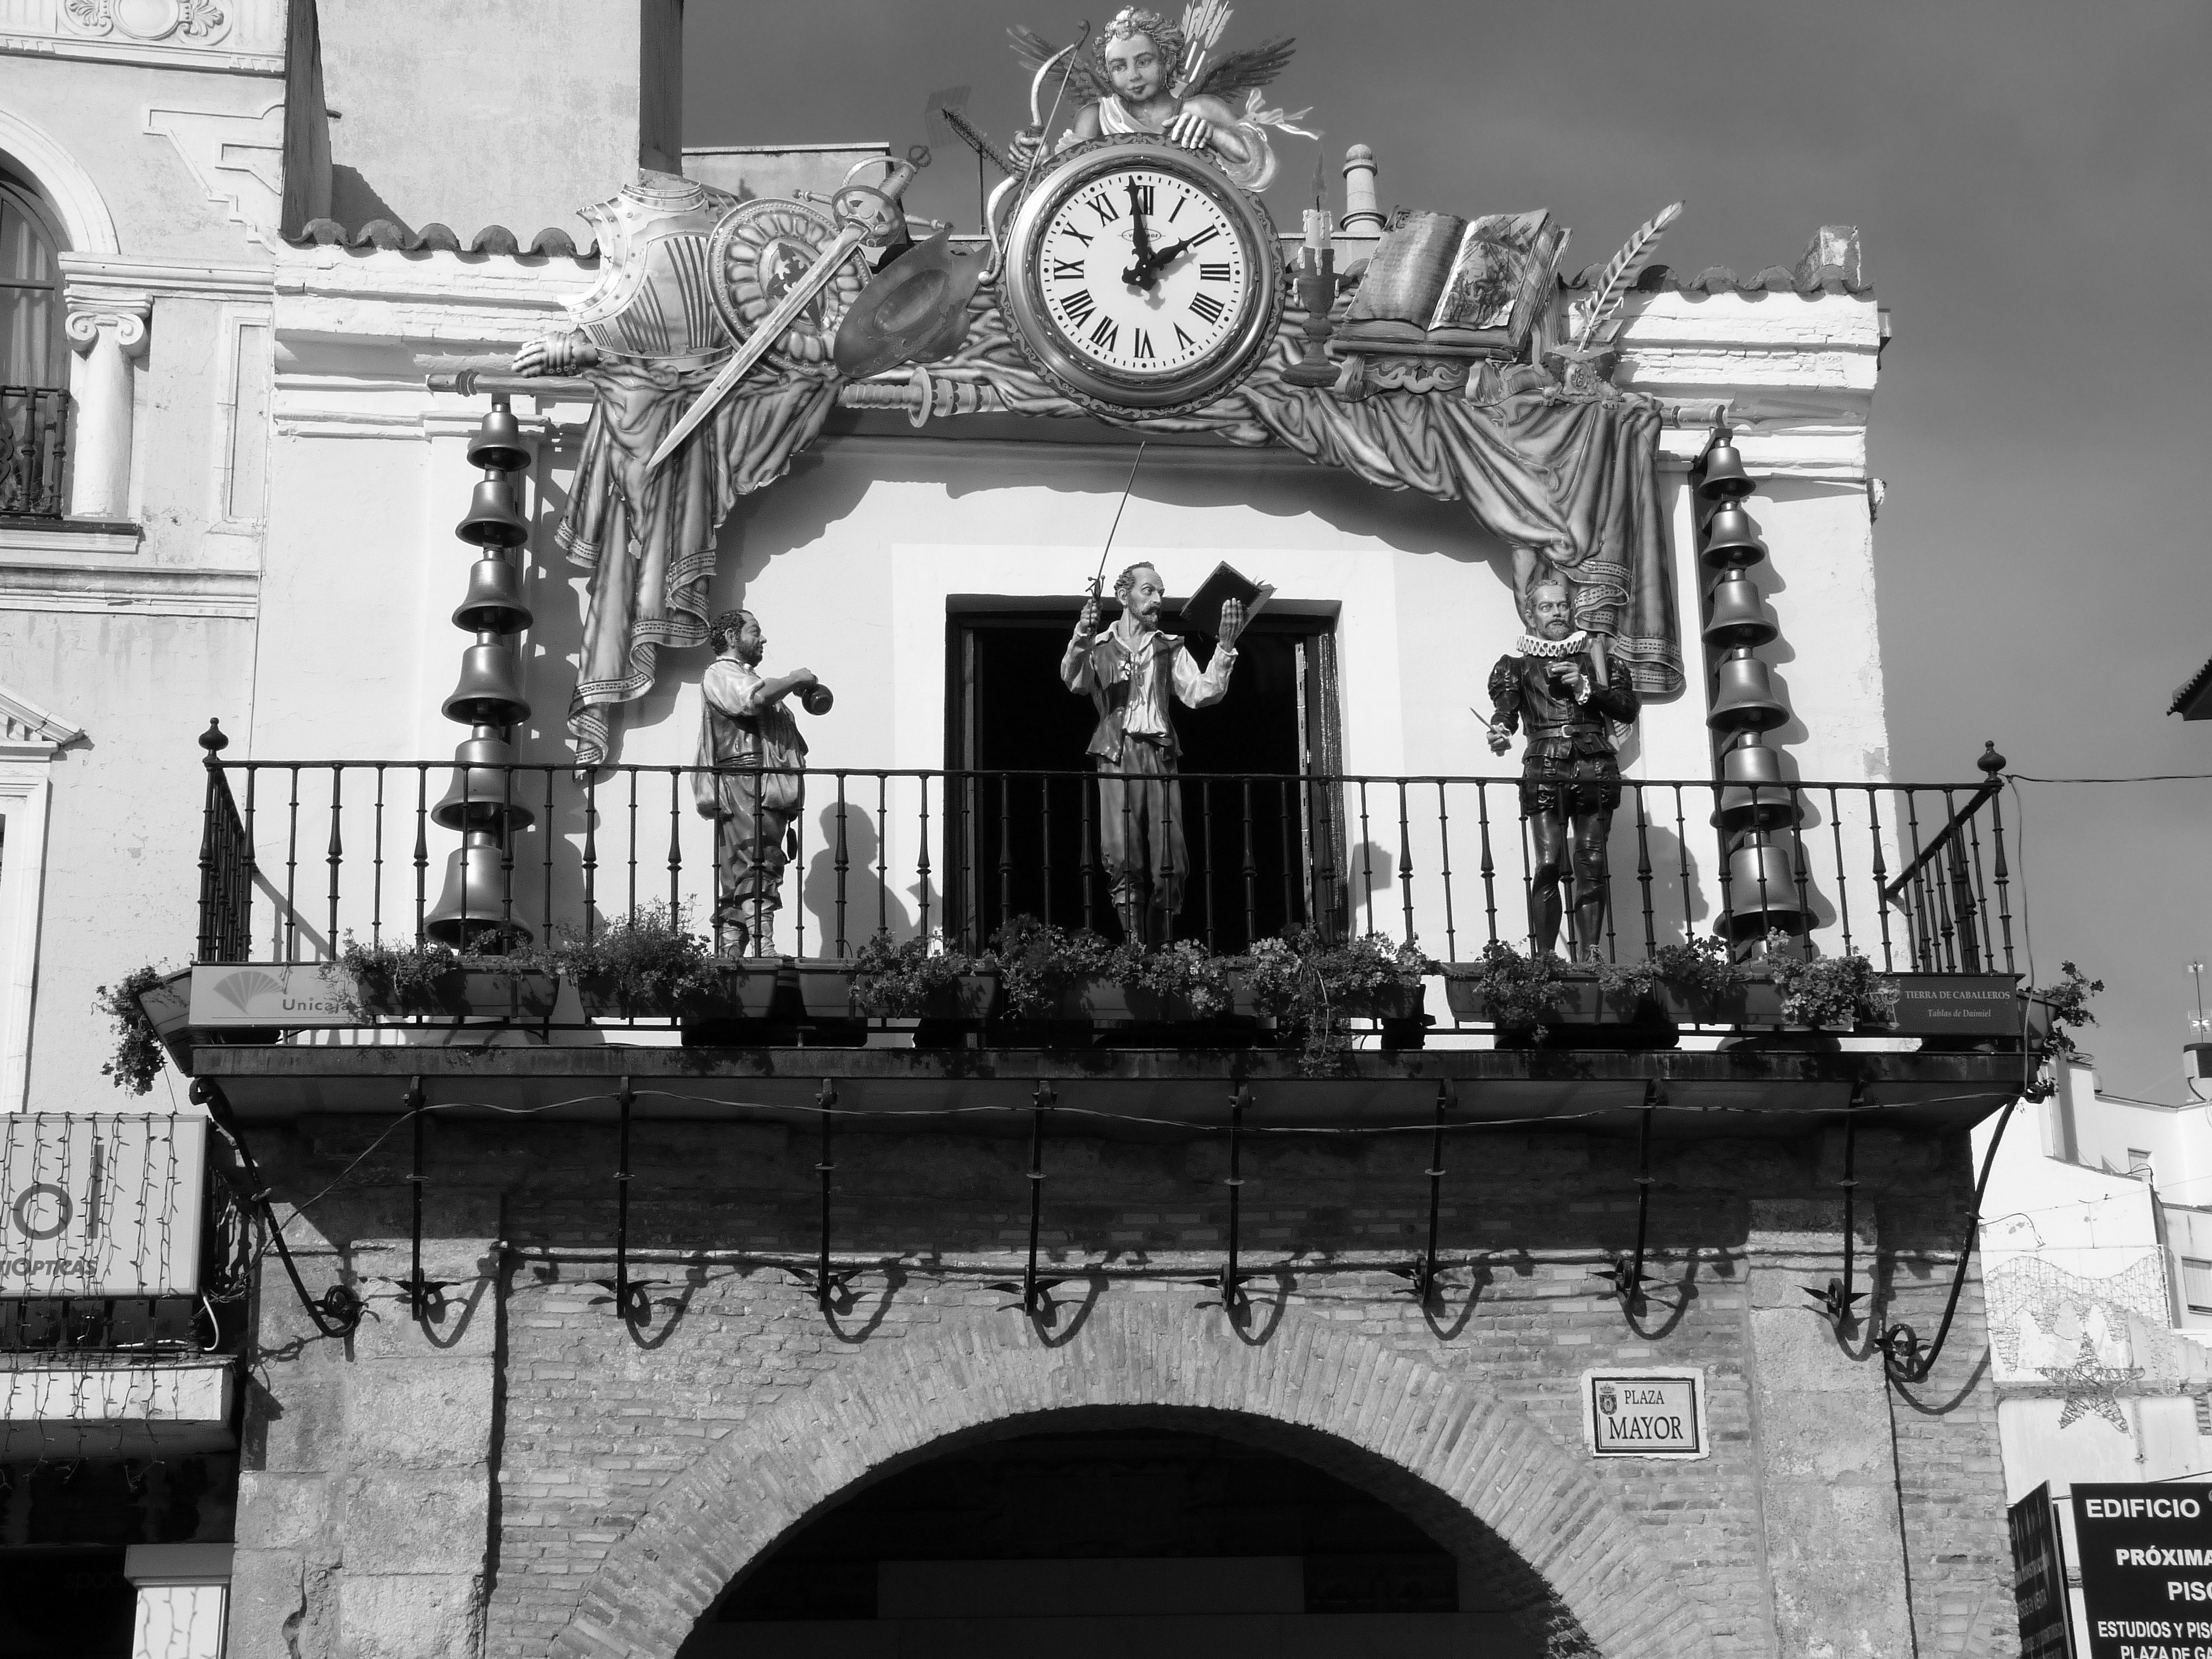
\includegraphics[width=0.8\linewidth]{./figs/clockCRbw}
		\caption{Fotografía en blanco y negro}\label{fig:fotoBW}
	\end{subfigure} 
	\caption[Ejemplo de subfiguras]{Ejemplo de inclusión de subfiguras en un mismo entorno (Fuente: J. Salido, \faCreativeCommons{} \faCreativeCommonsBy{} \faCreativeCommonsNcEu{} \faCreativeCommonsNd)}
	\label{fig:ejSubfigures}
\end{figure}

En los trabajos académicos la inclusión de imágenes y figuras que no son propiedad del autor suscitan bastante controversia. Ya que con frecuencia se incumple inadvertidamente la ley vigente de propiedad intelectual. Respecto a este hecho se recomienda, tanto a estudiantes como tutores, consultar documentación informativa sobre el uso correcto de figuras en documentos académicos \cite{uclm20,unican18}. Entre las <<incorrecciones>> más habituales en los documentos académicos, se observa:
\begin{itemize}
\item \emph{Abuso del derecho de cita}. Se produce al incluir, con fines exclusivamente decorativos o ilustrativos de la explicación, una figura sujeta a derechos de uso restringido invocando el derecho de cita (incluso con correcta atribución de la obra).

\item \emph{Incorrecta atribución de la obra}. Es habitual confundir al autor de la obra con la fuente de origen de la misma. La fuente es precisa cuando se cita la obra original. Sin embargo, la licencia de muchas obras exige la atribución al autor y la inclusión de la licencia bajo la que se distribuye o hace uso de la misma (véase como ejemplo cómo se realiza una correcta atribución en las Fig.~\ref{fig:ejFigure} y \ref{fig:ejSubfigures} mencionando al autor y la licencia Creative-Commons\footnote{\url{https://creativecommons.org}} bajo la que se rige el uso de la imagen y el mecanismo de título alternativo para que dicha atribución no aparezca en el índice de figuras usando título opcional).

\item \emph{Supresión de los detalles de la licencia de uso}. Al incluir obras de terceros debemos tener presente los términos de distribución de la misma e incluirlos junto a la atribución de su legítimo autor.
\end{itemize}

La inclusión de material de \emph{dominio público}, sin restricciones de uso o con permiso, hace innecesaria la atribución al autor, pero se recomienda incluir una nota de agradecimiento.\footnote{Incluyendo un texto como: \emph{<<Por cortesía de ...>>}}



\subsubsection{Algoritmos y listados de código fuente}
En los textos científicos relacionados con las 
TIC\footnote{Por supuesto, en un TFG (Trabajo Fin de Grado) o tesis 
de un centro superior de Informática.} (Tecnologías de la Información y 
Comunicaciones) suelen aparecer porciones de código en los que se explica 
alguna función o característica relevante del trabajo que se expone. Muchas 
veces lo que se quiere ilustrar es un algoritmo o método con el que se resuelve un problema abstrayéndose del lenguaje de implementación. El paquete \texttt{algorithm2e} proporciona un entorno \texttt{algorithm} para la impresión apropiada de algoritmos, tratándolos como objetos flotantes y con mucha flexibilidad de personalización, como se observa en el algoritmo~\ref{alg:como} del ejemplo.


% Ejemplo:
% ============
\IncMargin{1em}
\begin{algorithm}
\SetKwInOut{Input}{Datos}\SetKwInOut{Output}{Resultado}
\LinesNumbered
\SetAlgoLined

\Input{este texto} 
%\KwIn{este texto}
\Output{como escribir algoritmos con \LaTeX2e}
%\KwOut{como escribir algoritmos con \LaTeX2e}

inicialización\;
\While{no es el fin del documento}{
	leer actual\;
	\eIf{comprendido}{
		ir a la siguiente sección\;
		la sección actual es esta\;
	}{
		ir al principio de la sección actual\;
	}
}

% Aunque el captión aparece abajo siempre se pone arriba como en tablas y listados
\caption{Cómo escribir algoritmos}\label{alg:como}
\end{algorithm}\DecMargin{1em}








\newpage % Añadido para visualizar los listados completos en una página.
La inclusión de porciones de código fuente se puede formatear de modo sencillo en \LaTeX{} mediante el uso del paquete \texttt{listings}. A continuación, se muestran varios ejemplos de porciones de código correspondientes a distintos lenguajes de programación.


% Ejemplo: Listado Java
% ============
% Los entornos lstlisting se pueden tratar tambión como elementos flotantes mediante la opción 'float=hbt', donde se indica la ubicación del elemento.
\begin{lstlisting}[language=Java,caption={[Código fuente en Java]Ejemplo de código fuente en lenguaje Java},label=lst:java]
// @author www.javadb.com
public class Main {    
// Este método convierte un String a un vector de bytes

public void convertStringToByteArray() {

String stringToConvert = "This String is 15";      
	byte[] theByteArray = stringToConvert.getBytes();        
	System.out.println(theByteArray.length);        
}

public static void main(String[] args) {
	new Main().convertStringToByteArray();
}
}
\end{lstlisting}


\begin{lstlisting}[style=ruled,language=C,caption={Ejemplo de código fuente en lenguaje C},label=lst:codC]
// Este código se ha incluido tal cual está en el fichero \LaTeX{}
#include <stdio.h>

int main(int argc, char* argv[]) {
	puts("¡Hola mundo!");
}
\end{lstlisting}


\begin{lstlisting}[style=ruled,language=Matlab,caption={Ejemplo de script en Matlab},label=lst:matlab]
function f = fibonacci(n)
 % FIBONACCI  Fibonacci sequence
 %	f = FIBONACCI(n) generates the first n Fibonacci numbers.
 %	Copyright 2014 Cleve Moler
 %	Copyright 2014 The MathWorks, Inc.
f = zeros(n,1); 
f(1) = 1;
f(2) = 2;
for k = 3:n
f(k) = f(k-1) + f(k-2);
end
\end{lstlisting}



\subsubsection{Menús, paths y teclas con el paquete \texttt{menukeys}}
Cada vez es más usual que los trabajos en ingeniería exijan el uso de 
software. Para poder especificar de modo elegante el uso de menús, pulsación de 
teclas y directorios, se recomienda el uso del paquete 
\texttt{menukeys}.\footnote{\url{https://osl.ugr.es/CTAN/macros/latex/contrib/menukeys/menukeys.pdf}}
 \index{CTAN} Este paquete nos permite especificar el acceso a un menú, por 
ejemplo:\\

\noindent \menu{Herramientas:Órdenes:PDFLaTeX}\\

\noindent También un conjunto de teclas. Por ejemplo:
\keys{\ctrl + \shift + T}\\

\noindent O un directorio:
\directory{C:/user/LaTeX/Ejemplos}\\

\noindent Aunque este paquete permite muchas opciones de configuración de los estilos aplicados, no es necesario hacerlo para obtener unos resultados muy elegantes.


\subsection{Bibliografía}
Todo el material de terceros se debe citar convenientemente sin contravenir los términos de las licencias de uso y distribución de dicho material. Esto se extiende al uso de diagramas y fotografías. El incumplimiento de la legislación vigente en materia de protección de la propiedad intelectual es responsabilidad exclusiva del autor, independientemente de la cesión de derechos que este haya convenido.

La sección de \emph{Bibliografía}, que si se prefiere se puede titular \emph{Referencias}, incluirá un listado ordenado preferentemente por orden alfabético (primer apellido del autor principal), con todas las obras citadas en el texto. En la lista de referencias se especificará para cada obra: autores, título, editorial y año de publicación. Este formato se conseguirá en \LaTeX{} mediante el uso del estilo estándar \texttt{plain} o cualquier otro derivado con estilo de citación numérica. En algunas titulaciones se obliga a una ordenación por orden de cita en el texto que con Bib\TeX{} se puede obtener mediante los estilos estándar \texttt{ieeetr} (estilo para los IEEE \emph{transactions}) y \texttt{unsrt} (estilo \emph{unsorted}). 

Es muy importante tener presente que en esta sección solo se debe incluir las referencias bibliográficas citadas expresamente en el documento. Si se desea incluir fuentes consultadas, pero no citadas, se puede confeccionar con ellas una sección denominada \emph{Material de consulta}, aunque estas referencias se pueden incluir opcionalmente a lo largo del documento como notas a pie de página.

En las titulaciones técnicas se empleará estilo de citación numérico con el número de la referencia entre corchetes. La cita podrá incluir el número de página concreto de la referencia que se desea citar. El uso correcto de la citación implica dejar claro al lector cuál es el texto, material o idea citado. Las obras referenciadas sin mención explícita o implícita al material concreto citado se deberían considerar material de consulta y, por tanto, ser agrupadas como \emph{Material de consulta}, distinguiéndolas claramente de aquellas otras en las que si se recurre a la citación.

En las titulaciones que requieren un estilo de citación de tipo autor-año (no numérico), se puede incluir el paquete \LaTeX{} \texttt{apacite} (con la opción \texttt{natbibapa}) y especificar este mismo estilo en la sección de bibliografía en el argumento del comando \texttt{bibliographystyle}.

Cuando se desee incluir referencias a páginas genéricas de la Web sin mención expresa a un artículo con título y autor definido, dichas referencias se pueden incluir como notas al pie de página o como un apartado de fuentes de consulta dedicado a \emph{Direcciones de Internet}. Por el contrario, los documentos electrónicos publicados en Internet se pueden incluir empleando el tipo de entrada \texttt{misc} como se muestra en la bibliografía que acompaña esta plantilla.





\chapter{Objetivo}
\label{cap:Objetivo}
Este es un capítulo en el que se determina de modo claro el objetivo general del trabajo descrito que se puede desglosar en objetivos secundarios cuando el objetivo principal se descompone en módulos o componentes. 

Es muy importante definir el objetivo de modo apropiado. Debe concretar y exponer detalladamente el problema a resolver, el entorno de trabajo, la situación y qué se pretende obtener. También puede contemplar las limitaciones y condicionantes a considerar para la resolución del problema (lenguaje de construcción, equipo físico, equipo lógico de base o de apoyo, 
etc.).


\section{Cómo plantear el objetivo de un TFG en ingeniería}
Una de las tareas más complicadas al proponer un TFG es plantear su \textsf{Objetivo}. La dificultad deriva de la falta de consenso respecto de lo que se entiende por \emph{objetivo} en un trabajo de esta naturaleza. En primer lugar, se debe distinguir entre dos tipos de objetivo:


\begin{enumerate}[(A)]
	\item La \emph{finalidad específica} del TFG que se plantea para resolver una problemática concreta aplicando los métodos y herramientas adquiridos durante la formación académica. Por ejemplo, \emph{<<Desarrollo de una aplicación software para gestionar reservas hoteleras \emph{on-line}>>}.
	
	\item El \emph{propósito académico} que la realización de un TFG tiene en la formación de un graduado. Por ejemplo, la \emph{adquisición de competencias específicas de la especialización} cursada.
\end{enumerate}

En el ámbito de la memoria del TFG se tiene que definir el primer tipo de objetivo, mientras que el segundo tipo es el que se añade al elaborar la propuesta de un TFG presentada ante un comité para su aprobación. \emph{Este segundo tipo de objetivo no se debe incluir en la memoria y en todo caso hacerse en la sección de conclusiones finales.}\footnote{En algunas titulaciones es obligatorio que la memoria explique las competencias específicas alcanzadas con la realización del trabajo.}

Un objetivo bien planteado debe estar determinado en términos del \emph{<<producto final>>} esperado que resuelve un problema específico. Por tanto, debería quedar determinado por un sustantivo \emph{concreto} y \emph{medible}. El objetivo planteado puede pertenecer a una de las categorías que se indica a continuación:
\begin{itemize}
	\item \emph{Diseño y desarrollo de <<artefactos>>}
	(habitual en las ingenierías). Por la naturaleza de los programas informáticos (software), los trabajos que implican su diseño suelen contemplar también el desarrollo o implementación de prototipos. Esto es menos frecuente en otras áreas de ingeniería en las que claramente se separa la fase de diseño o realización de un proyecto, frente a la ejecución del mismo (p.~ej.,~ingeniería civil, arquitectura, etc.). 
    
	\item \emph{Estudio} que ofrece información novedosa sobre un tema (usual en las ramas de ciencias y humanidades). 
    
	\item \emph{Validación de una 
	hipótesis} de partida (propio de los trabajos 
	científicos y menos habitual en el caso de los TFG).
\end{itemize}

Estas categorías no son excluyentes, de modo que es posible plantear un trabajo cuyo objetivo sea el diseño y desarrollo de un <<artefacto>> y este implique un estudio previo o la validación de alguna hipótesis para guiar el proceso. En este caso y cuando el objetivo sea lo suficientemente amplio puede ser conveniente su descomposición en elementos más simples hablando de \emph{subobjetivos}. Por ejemplo, un programa informático se puede descomponer en módulos o requerir un estudio previo para plantear un nuevo algoritmo que será preciso validar. La descomposición de un objetivo principal en subobjetivos 
u objetivos secundarios debería ser natural (no forzada), bien justificada y 
sólo pertinente en los trabajos de gran amplitud.

Junto con la definición del objetivo del trabajo se puede especificar los \emph{requisitos} que debe satisfacer la solución aportada. Estos requisitos especifican \emph{características} que debe poseer la solución y \emph{restricciones} que acotan su alcance. En el caso de un trabajo cuyo objetivo es el desarrollo de un <<artefacto>> los requisitos pueden ser \emph{funcionales} y \emph{no funcionales}.

Al redactar el objetivo de un TFG se puede confundir los medios con el 
fin. De este modo es posible encontrarse con objetivos definidos en términos de las 
\emph{acciones} (verbos) o \emph{tareas} que será preciso 
realizar para alcanzar el resultado deseado. Aunque deben evitarse en la definición del objetivo del TFG, a la hora de 
planificar el desarrollo del trabajo, si es apropiado descomponer su elaboración en \emph{hitos} y estos en \emph{tareas} que faciliten su 
\emph{planificación}.

La categoría del objetivo planteado justifica modificaciones en la organización genérica de la memoria del trabajo. Así en el caso de estudios y validación de hipótesis el apartado de resultados y conclusiones debería incluir los resultados de experimentación y los comentarios de cómo dichos resultados validan o refutan la hipótesis planteada.


\chapter{Metodología}
\label{cap:Metodologia}

En este capítulo se debe detallar las metodologías
empleadas para planificación y desarrollo del trabajo, así como explicar de 
modo claro y conciso cómo se han aplicado dichas metodologías.

A continuación se incluye una guía rápida que puede ser de gran utilidad en la elaboración de este capítulo.

\section{Guía rápida de las metodologías de desarrollo de software}

\subsection{Proceso de desarrollo de software}

El \textbf{proceso de desarrollo de software} se denomina también 
\textbf{ciclo de vida del desarrollo del software} (\emph{SDLC, Software 
Development Life-Cycle}) y cubre las siguientes 
actividades:

\begin{enumerate}[1.-]
\item \textbf{Obtención y análisis de requisitos}
(\emph{requirements analysis}). Es la definición de la funcionalidad del 
software a desarrollar. Suele requerir entrevistas entre los ing. de software 
y el cliente para obtener el `qué' y `cómo'. Permite obtener una 
\emph{especificación funcional} del software.

\item \textbf{Diseño} (\emph{SW design}). Consiste en la 
definición de la arquitectura, los componentes, las interfaces y otras 
características del sistema o sus componentes.

\item \textbf{Implementación} (\emph{SW construction and coding}). Es el
  proceso de codificación del software en un lenguaje de programación.
  Constituye la fase en que tiene lugar el desarrollo de software.

\item \textbf{Pruebas} (\emph{testing and verification}).
Verificación del correcto funcionamiento del software para detectar fallos lo 
antes posible. Persigue la obtención de software de calidad. Consisten en 
pruebas de \emph{caja negra} y \emph{caja blanca}. Las primeras comprueban 
que la funcionalidad es la esperada y para ello se verifica que ante un 
conjunto amplio de entradas, la salida es correcta. Con las segundas se 
comprueba la robustez del código sometiéndolo a pruebas cuya finalidad es 
provocar fallos de software. Esta fase también incorpora la \emph{pruebas de 
integración} en las que se verifica la interoperabilidad del sistema con 
otros existentes.

\item \textbf{Documentación} (\emph{documentation}). Persigue facilitar la mejora continua del software y su mantenimiento.

\item \textbf{Despliegue} (\emph{deployment}). Consiste en 
la instalación del software en un entorno de producción y puesta en marcha 
para explotación. En ocasiones implica una fase de \emph{entrenamiento} de 
los usuarios del software.

\item \textbf{Mantenimiento} (\emph{maintenance}). Su 
propósito es la resolución de problemas, mejora y adaptación del software en 
explotación.
\end{enumerate}




\subsection{Metodologías de desarrollo software}
\emph{Las metodologías son el modo en que las fases del proceso software se organizan e interaccionan para conseguir que dicho proceso sea reproducible y predecible para aumentar la productividad y la calidad del software.}

Una metodología es una colección de:

\begin{enumerate}[A.]
\item \textbf{Procedimientos} (indican cómo hacer cada tarea y en qué momento),
\item \textbf{Herramientas} (ayudas para la realización de cada tarea), y
\item \textbf{Ayudas documentales}.
\end{enumerate}

Cada metodología es apropiada para un tipo de proyecto dependiendo de sus 
características técnicas, organizativas y del equipo de trabajo. En los 
entornos empresariales es obligado, a veces, el uso de una metodología 
concreta (p.~ej. para participar en concursos públicos). El estándar 
internacional ISO/IEC 12270 describe el método para 
seleccionar, implementar y monitorear el ciclo de vida del software.

Mientras que unas intentan sistematizar y formalizar las tareas de diseño, otras aplican técnicas de gestión de proyectos para dicha tarea. Las metodologías de desarrollo se pueden agrupar dentro de varios enfoques según se señala a continuación.

\begin{enumerate}
\item \textbf{Metodología de Análisis y Diseño de Sistemas Estructurados} 
(\emph{SSADM, Structured Systems Analysis and Design 
Methodology}). Es uno de los paradigmas más antiguos. En esta 
metodología se emplea un modelo de desarrollo en cascada 
(\emph{waterfall}). Las fases de 
desarrollo tienen lugar de modo secuencial. Una fase comienza cuando termina 
la anterior. Es un método clásico poco flexible y adaptable a cambios en los 
requisitos. Hace especial hincapié en la planificación derivada de una 
exhaustiva definición y análisis de los requisitos. Son metodologías que no 
lidian bien con la flexibilidad requerida en los proyectos de desarrollo 
software. Derivan de los procesos en  ingeniería tradicionales y están 
enfocadas a la reducción del riesgo. Emplea tres técnicas clave:

\begin{itemize}
\item Modelado lógico de datos (\emph{Logical Data 
Modelling}),
\item Modelado de flujo de datos (\emph{Data Flow Modelling}), y
\item Modelado de Entidades y Eventos (\emph{Entity Event
  Modelling}).
\end{itemize} 

\item \textbf{Metodología de Diseño Orientado a Objetos} (\emph{OOD,  
Object-Oriented Design}). Está muy ligado a la OOP (Programación 
Orientada a Objetos) en que se persigue la reutilización. A diferencia del 
anterior, en este paradigma los datos y los procesos se combinan en una única 
entidad denominada \emph{objetos} (o clases). Esta orientación pretende que 
los sistemas sean más modulares para mejorar la eficiencia, calidad del 
análisis y el diseño. Emplea extensivamente el Lenguaje Unificado de Modelado 
(UML) para especificar, visualizar, construir y documentar los 
artefactos de los sistemas software y  también el modelo de negocio. UML 
proporciona una serie diagramas de básicos para modelar un sistema: 

\begin{itemize}
\item Diagrama de Clase (\emph{Class Diagram}). Muestra los objetos del sistema y sus relaciones. 
\item Diagrama de Caso de Uso (\emph{Use Case Diagram}). Plasma la
  funcionalidad del sistema y quién interacciona con él.
\item Diagrama de secuencia (\emph{Sequence Diagram}). Muestra los eventos que se
  producen en el sistema y como este reacciona ante ellos. 
\item Modelo de Datos (\emph{Data Model}).
\end{itemize} 
                               
\item \textbf{Desarrollo Rápido de Aplicaciones} (\emph{RAD, Rapid 
Application Developmnent}). Su filosofía es sacrificar calidad a 
cambio de poner en producción el sistema rápidamente con la funcionalidad 
esencial. Los procesos de especificación, diseño e implementación son 
simultáneos. No se realiza una especificación detallada y se reduce la 
documentación de diseño. El sistema se diseña en una serie de pasos, los 
usuarios evalúan cada etapa en la que proponen cambios y nuevas mejoras. Las 
interfaces de usuario se desarrollan habitualmente mediante sistemas 
interactivos de desarrollo. En vez de seguir un modelo de desarrollo en 
cascada sigue un modelo en espiral (Boehm). La clave de 
este modelo es el desarrollo continuo que ayuda a minimizar los riesgos. Los 
desarrolladores deben definir las características de mayor prioridad. Este 
tipo de desarrollo se basa en la creación de prototipos y realimentación 
obtenida de los clientes para definir e implementar más características hasta 
alcanzar un sistema aceptable para despliegue.

\item \textbf{Metodologías Ágiles}. \emph{"[...] envuelven un enfoque para la 
toma de decisiones en los proyectos de software, que se refiere a métodos de 
ingeniería del software basados en el desarrollo iterativo e incremental, 
donde los requisitos y soluciones evolucionan con el tiempo según la 
necesidad del proyecto. Así el trabajo es realizado mediante la colaboración 
de equipos auto-organizados y multidisciplinarios, inmersos en un proceso 
compartido de toma de decisiones a corto plazo. Cada iteración del ciclo de 
vida incluye:  planificación, análisis de requisitos, diseño, codificación, 
pruebas y  documentación. Teniendo gran importancia el concepto de 
"Finalizado" (Done), ya que el objetivo de cada iteración no es agregar toda 
la funcionalidad para justificar el lanzamiento del producto al mercado, sino 
incrementar el valor por medio de "software que funciona" (sin errores). Los 
métodos ágiles enfatizan las comunicaciones cara a cara en vez de la 
documentación. [...]"}\footnote{Fuente: Wikipedia}
\end{enumerate}

\subsection{Proceso de testing}

\begin{enumerate}
\item \emph{Pruebas modulares} (pruebas unitarias). Su propósito es hacer pruebas sobre un módulo tan pronto como sea posible. Las \emph{pruebas unitarias} que comprueban el correcto funcionamiento de una unidad de código. Dicha unidad elemental de código consistiría en cada función o procedimiento, en el caso de programación estructurada y cada clase, para la programación orientada a objetos. Las características de una prueba unitaria de calidad son: \emph{automatizable} (sin intervención manual), \emph{completa},  \emph{reutilizable}, \emph{independiente} y \emph{profesional}.

\item \emph{Pruebas de integración}. Pruebas de varios módulos en conjunto para comprobar su interoperabilidad.

\item \emph{Pruebas de caja negra}.

\item \emph{Beta testing}.

\item \emph{Pruebas de sistema y aceptación}.

\item \emph{Training}.
\end{enumerate}






\subsection{Herramientas CASE (\emph{Computer Aided Software Engineering})}

Las herramientas CASE están destinadas a facilitar una o varias 
de las tareas implicadas en el ciclo de vida del desarrollo de software. Se 
pueden dividir en la siguientes categorías:

\begin{enumerate}
\item Modelado y análisis de negocio.
\item Desarrollo. Facilitan las fases de diseño y construcción.
\item Verificación y validación.
\item Gestión de configuraciones.
\item Métricas y medidas.
\item Gestión de proyecto. Gestión de planes, asignación de tareas, planificación, etc.
\end{enumerate}




\subsubsection{IDE (Integrated Development Environment)}
\begin{multicols}{2}
\begin{itemize}[nosep]
\item \href{https://notepad-plus-plus.org/}{Notepad++}
\item \href{https://code.visualstudio.com/}{Visual Studio Code}
\item \href{https://atom.io/}{Atom}
\item \href{https://www.gnu.org/s/emacs/}{GNU Emacs}
\item \href{https://netbeans.org/}{NetBeans}
\item \href{https://eclipse.org/}{Eclipse}
\item \href{https://www.qt.io/ide/}{Qt Creator}
\item \href{http://www.jedit.org/}{jEdit}
\item \href{https://www.jetbrains.com/idea/}{ItelliJ IDEA}
\end{itemize}
\end{multicols}



\subsubsection{Depuración}
\begin{itemize}[nosep]
\item \href{https://www.gnu.org/s/gdb/}{GNU Debugger}
\end{itemize}


\subsubsection{Testing}
\begin{multicols}{2}
\begin{itemize}[nosep]
\item \href{http://junit.org}{JUnit}. Entorno de pruebas para Java.
\item \href{http://cunit.sourceforge.net/}{CUnit}. Entorno de pruebas para C.
\item \href{https://wiki.python.org/moin/PyUnit}{PyUnit}. Entorno de pruebas para Python.
\end{itemize}
\end{multicols}

\subsubsection{Repositorios y control de versiones}
\begin{multicols}{2}
\begin{itemize}[nosep]
\item \href{https://git-scm.com/}{Git}
\item \href{https://www.mercurial-scm.org/}{Mercurial}
\item \href{https://github.com/}{Github}
\item \href{https://bitbucket.org/}{Bitbucket}
\item \href{https://www.sourcetreeapp.com/}{SourceTree}
\end{itemize}
\end{multicols}


\subsubsection{Documentación}
\begin{multicols}{2}
\begin{itemize}[nosep]
\item \href{https://www.latex-project.org/}{\LaTeX}
\item \href{https://markdown.es/}{Markdown}
\item \href{http://www.stack.nl/\%7Edimitri/doxygen/index.html}{Doxygen}
\item \href{http://mtmacdonald.github.io/docgen/docs/index.html}{DocGen}
\item \href{http://pandoc.org/}{Pandoc}
\end{itemize}
\end{multicols}



\subsubsection{Gestión y planificación de proyectos}
\begin{multicols}{2}
\begin{itemize}[nosep]
\item \href{https://trello.com/}{Trello}
\item \href{https://es.atlassian.com/software/jira}{Jira}
\item \href{https://asana.com/}{Asana}
\item \href{https://slack.com/}{Slack}
\item \href{https://basecamp.com/}{Basecamp}
\item \href{https://www.teamwork.com/project-management-software}{Teamwork Projects}
\item \href{https://www.zoho.com/projects/}{Zoho Projects}
\end{itemize}
\end{multicols}


\subsection{Fuentes de información adicional}
\begin{itemize}[nosep]
\item \href{https://leankit.com/blog/2019/03/top-6-software-development-methodologies/}{Top
  6 Software Development Methodologies}. Maja Majewski. Planview
  LeanKit, 2019.
\item \href{https://acodez.in/12-best-software-development-methodologies-pros-cons/}{12
  Best software development methodologies with pros and cons}. acodez,
  2018.
\item \href{http://www.itinfo.am/eng/software-development-methodologies/}{Software
  Development Methodologies}. Association of Modern Technologies
  Professionals, 2019.
\end{itemize}

\chapter{Resultados}
\label{cap:Resultados}

En esta sección se describirá la aplicación del método de trabajo presentado en el capítulo \ref{cap:Metodologia},  mostrando los elementos (modelos, diagramas, especificaciones, etc.) más importantes. 

Este apartado debe explicar cómo el empleo de la metodología permite satisfacer tanto el objetivo principal como los específicos planteados en el TFG así como los requisitos exigidos (según exposición en cap.~\ref{cap:Objetivo}).
\chapter{Conclusiones}
\label{cap:Conclusiones}

En este capítulo se realizará un juicio crítico y discusión sobre los resultados obtenidos. \emph{Cuidado, esta discusión no debe confundirse con una valoración del enriquecimiento personal que supone la realización del trabajo como culminación de una etapa académica}. Aunque de gran importancia, esta última valoración debe quedar fuera de la memoria del trabajo y solo debe ahondarse en ella ante requerimiento explícito del comité en el acto de defensa.

Si es pertinente deberá incluir información sobre trabajos derivados como publicaciones o ponencias en preparación, así como trabajos futuros \emph{(solo si estos están iniciados o planificados en el momento que se redacta el texto)}. Evitar hacer una lista de posibles mejoras. Contrariamente a lo que alguno pueda pensar generalmente aportan impresión de trabajo incompleto o inacabado.\footnote{Puede reflexionarse en ello por si en la defensa del trabajo se pregunta sobre estas posibles mejoras.}


\section{Justificación de competencias adquiridas}
Es muy importante recordar que según la normativa vigente en la ESI-UCLM, el capítulo de conclusiones debe incluir \emph{obligatoriamente} un apartado destinado a justificar la aplicación en el TFG de las competencias específicas (una o más) adquiridas en la tecnología específica cursada.

En el TFG se han aplicado las competencias correspondientes a la Tecnología Específica de \emph{[poner lo que corresponda]}:

\begin{description}
\item[Código de la competencia 1:] \emph{[Texto de la competencia 1]}. Explicación de cómo se ha aplicado en el TFG.
\item[\dots] otras más si las hubiera.
\end{description}







%--- (FIN FRONTMATTER)







% -------------------------
% No olvides retornar al interlineado sencillo en el resto del documento.
\singlespacing
% -------------------------
% -------------------------
% -------------------------
% -------------------------
%
%--- BACKMATTER
%BEGIN_FOLD
% \backmatter 
% Comentado para que apéndices aparezcan numerados después de la bibliografía


% -------------------------
% --- BIBLIOGRAFÍA
% -------------------------
\cleardoublepage % Necesario para ajustar el avance de página
\phantomsection  % Ojo necesario con hyperref.
\addcontentsline{toc}{chapter}{\bibname} % Añade la bibliografía al Índice de contenidos

% EDITAR: Definición del estilo empleado en la bibliografía
% Comentar si se emplea lista de \bibitem{citekey}
\bibliographystyle{plain}
% Estilos nativos incluidos con LaTeX (plain, abbrv, alpha, unsrt).
%
% plain: las referencias se numeran y en la bibliografía las entradas
%        aparecen en orden alfabético.
% abbrv: igual que el anterior pero en la bibliografía los nombres se
%        escriben sólo con la inicial.
%        y el año de publicación. En la bibliografía los nombres 
%        igual que en plain. 
%        .
% unsrt: la bibliografía no aparece por orden alfabético sino por 
%        orden de cita en el texto.

% Estilos incluidos con BibTeX “no nativos” pero muy “populares” para ingenierías
%
% acm:       Numérica con los nombre de autores en mayúsculas y referencias con
%            ordenación alfabética.
% ieeetr:    Para los IEEE Transactions, con citación numérica y ordenación de 
%            referencias por orden de cita.
% apacite:   No numérica, con referencias ordenadas alfabéticamente por apellido %            de autor.
%---
% Comentar si se emplea lista de \bibitem{citekey} 
\bibliography{biblioTFG} % Nombre del fichero .bib (sin extensión)
% -------------------------

% -------------------------
% Sustituir por entorno 
% Contenido obtenido de fichero auxiliar bbl donde de puede editar
% manualmente cada una de las entradas.
%\begin{thebibliography}{10}
%\bibitem{borbon21}
%Alexánder Borbón and Walter Mora.
%\newblock {\em Edición de textos científicos con {\LaTeX{}}. {C}omposición,
%  diseño editorial, gráficos, {I}nkscape, {T}ikz y presentaciones {B}eamer}.
%\newblock Instituto Tecnológico de Costa Rica, 2 edition, 2021.
%
%\bibitem{cascales03}
%Bernardo Cascales, Pascual Lucas, José~M. Mira, Antonio~J. Pallarés, and
%  Salvador {Sánchez-Pedreño}.
%\newblock {\em El libro de {\LaTeX}}.
%\newblock Pearson Education, 2005.
%\newblock {ISBN}: 9788420537795.
%
%\bibitem{esi19}
%{Escuela Superior de Informática, Universidad de Castilla-La Mancha}.
%\newblock Guía de estilo y formato para {T}rabajos {F}in de {G}rado.
%\newblock {URL:}
%  \url{https://pruebasaluuclm.sharepoint.com/sites/esicr/tfg/SiteAssets/SitePages/Inicio/20190304-GuiaEstiloFormatoTFG.pdf},
%  March 2019.
%\newblock Último acceso: sep. 2021.
%
%\bibitem{goos07}
%Michel Goossens, Frank Mittelbach, Sebastian Rahtz, Denis Roeget, and Herbert
%  Vo{\ss}.
%\newblock {\em The {\LaTeX{}} graphics companion}.
%\newblock Addison-Wesley Reading, MA, second edition, 2007.
%\newblock {ISBN:} 9780321508928.
%
%\bibitem{grat99}
%George~A. Grätzer.
%\newblock {\em First steps in {\LaTeX}}.
%\newblock Springer Verlag, October 1999.
%\newblock {ISBN:} 0817641327.
%
%\bibitem{grat07}
%George~A. Grätzer.
%\newblock {\em More math into {\LaTeX}}.
%\newblock Birkhauser, fourth edition, 2007.
%\newblock {ISBN}: 978-3319237954.
%
%\bibitem{lamport94}
%Leslie Lamport.
%\newblock {\em {\LaTeX}: A document preparation system}.
%\newblock Addison-Wesley, second edition, June 1994.
%\newblock {ISBN}: 978-0201529838.
%
%\bibitem{mittelbach04}
%Frank Mittelbach and Michel Goossens.
%\newblock {\em The {\LaTeX{}} companion}.
%\newblock Addison, Reading, Mass, second edition, 2004.
%\newblock {ISBN:} 0-201-36299-6.
%
%\bibitem{oetiker14}
%Tobias Oetiker, Hubert Partl, Irene Hyna, and Elisabeth Schlegl.
%\newblock {\em La introducción no-tan-corta a {\LaTeX2e}}, 2014.
%
%\bibitem{salido10}
%Jesús Salido.
%\newblock Curso: {\LaTeX{}} esencial para preparación de tfg, tesis y otros
%  documentos académicos.
%\newblock {URL:} \url{http://visilab.etsii.uclm.es/?page_id=1468}, 2010.
%\newblock Último acceso: sep. 2021.
%
%\bibitem{salido19}
%Jesús Salido.
%\newblock {Plantilla LaTeX para Trabajo Fin de Estudios en Ingeniería
%  Informática - UCLM (España)}.
%\newblock Zenodo, DOI: \url{https://doi.org/10.5281/zenodo.4561708}, 2019.
%
%\bibitem{uclm20}
%{Servicio de publicaciones UCLM}.
%\newblock Propiedad intelectual.
%\newblock {D}ocumentos elaborados por el {G}rupo de {G}estión del
%  {C}onocimiento y {P}ropiedad {I}ntelectual de la {Universidad de Castilla-La
%  Mancha}. {URL:} \url{https://publicaciones.uclm.es/propiedad-intelectual/}.
%\newblock Último acceso: jun. 2022.
%
%\bibitem{uc3m21}
%{Universidad Carlos III de Madrid}.
%\newblock Guía temática del {TFG}.
%\newblock {URL:} \url{https://uc3m.libguides.com/TFG}, 2021.
%\newblock Último acceso: sep-2021.
%
%\bibitem{unican18}
%{Universidad de Cantabria}.
%\newblock Cómo usar imágenes en trabajos.
%\newblock Artículo técnico disponible en {URL:}
%  \url{https://web.unican.es/buc/Documents/Formacion/guia_imagenes.pdf}, 2018.
%\newblock Último acceso: sep. 2021.
%
%\bibitem{uoc}
%{Universitat Oberta de Catalunya}.
%\newblock Comunicación eficaz y redacción.
%\newblock {URL:}
%  \url{https://www.uoc.edu/portal/es/servei-linguistic/redaccio/10-recomanacions/index.html}.
%\newblock Último acceso: sep. 2021.
%
%\bibitem{Vijayasarathy_2016}
%Leo~R. Vijayasarathy and Charles~W. Butler.
%\newblock {Choice of Software Development Methodologies: Do Organizational,
%  Project, and Team Characteristics Matter?}
%\newblock {\em {IEEE} Software}, 33(5):86--94, sep 2016.
%
%\bibitem{wikibookLaTex10}
%WikiMedia.
%\newblock {\LaTeX{} Wikibook}.
%\newblock {URL:} \url{http://en.wikibooks.org/wiki/LaTeX}, 2010.
%\newblock Último acceso: sep. 2021.
%
%\bibitem{zozaya17}
%Leonor Zozaya.
%\newblock Redacción de textos. recomendaciones para presentar trabajos
%  académicos.
%\newblock Blog disponible en {URL:} \url{http://redaccion.hypotheses.org/},
%  2017.
%\newblock {ISSN}: 2444-8885.
%\end{thebibliography}
  





% -------------------------
% - ANEXOS: Comentar si no se desean incluir. [OPT.]
% - Mover si se desea que aparezcan antes de la bibliografía.
% -------------------------
\appendix
\ifspanish
	\part*{\sffamily ANEXOS}
\else
	\part*{\sffamily APPENDICES}
\fi
% Tras este punto los capítulos se numeran con letras.
% Aquí todos los apéndices necesarios
\chapter{El primer anexo}
\label{cap:AnexoA}

Los anexos se incluirá de modo opcional material suplementario que podrá consistir en breves manuales, listados de código fuente, esquemas, planos, etc. Se recomienda que no sean excesivamente voluminosos, aunque su extensión no estará sometida a regulación por afectar esta únicamente al texto principal. 




 % Apéndice A (opcionales)

%END_FOLD
%--- (FIN DOCUMENTO)
\end{document}